\documentclass{beamer}

\mode<presentation>{
  \usetheme{puc}
  \usecolortheme{beaver}
  \setbeamertemplate{caption}[numbered]
}

\usepackage[utf8]{inputenc}
\usepackage[brazilian]{babel}
\uselanguage{Brazilian}
\languagepath{Brazilian}
\usepackage{hyperref}
\usepackage{mathtools}
\usepackage{listings}
\usepackage{color}
\usepackage[normalem]{ulem}
\usepackage{textcomp}
\usepackage{adjustbox}
\usepackage{booktabs}
\usepackage{subfigure}
\usepackage{tikz}
\usetikzlibrary{arrows,calc,positioning,shadows,shapes,trees}
\newdimen\hdim                  % element height
\newdimen\wdim                  % element width
\newdimen\odim                  % offset distance
\hdim=2.25em
\wdim=2.36\hdim
\odim=\hdim
\tikzstyle{element}=[
  draw=black!60,
  font={\scriptsize\sffamily},
  inner sep=0pt,
  minimum height=\hdim,
  minimum width=\wdim,
  outer sep=0pt,
  rectangle,
  rounded corners=\wdim/10,
  text centered,
  thick,
  top color=white,
  bottom color=black!20,
]
\tikzstyle{arrow}=[
  color=black!60,
  draw=black!60,
  thick,
]
\tikzstyle{arrowlabel}=[
  color=black!60,
  font={\tiny\sffamily\bfseries},
]
\tikzstyle{bin}=[
  dashed,
  draw=black!60,
  font={\tiny\sffamily\bfseries},
  rounded corners=\wdim/12,
]
\tikzstyle{binlabel}=[
  anchor=west,
  color=black!60,
  inner sep=0pt,
  outer sep=0pt,
  pos=0,
  xshift=.25em,
  yshift=-.45em,
]
\tikzstyle{state}=[
  circle,
  draw,
  font={\scriptsize\sffamily},
  inner sep=0pt,
  minimum height=1.5\hdim,
  minimum width=1.5\hdim,
  text width=\hdim,
  outer sep=0pt,
  text centered,
]
\tikzstyle{keystroke}=[
  draw,
  drop shadow={
    shadow xshift=0.25ex,
    shadow yshift=-0.25ex,
    fill=black,
    opacity=0.75,
  },
  fill=white,
  font=\scriptsize\sffamily,
  inner sep=2.5pt,
  line width=0.5pt,
  minimum width={1.7em},
  rectangle,
  rounded corners=2pt,
]
\tikzset{
  node distance=\wdim+\odim,
  >=stealth,
  shorten >=.5pt,
}

\newcommand*\keystroke[1]{%
  \tikz[baseline=(key.base)]\node[keystroke](key) {#1\strut};
}

\let\C\lstinline
\def\<#1>{\ensuremath{\left<#1\right>}}

\def\en#1{\foreignlanguage{english}{\emph{#1}}}

\lstset{
  basicstyle=\footnotesize\ttfamily,
  keywordstyle=\bfseries,
  breaklines=false,
  keepspaces=true,
  abovecaptionskip=0pt,
  aboveskip=\smallskipamount,
  belowcaptionskip=0pt,
  belowskip=\smallskipamount,
  captionpos=b,
  numbers=left,
  numberstyle=\tiny,
  numbersep=5pt,
  upquote,
  escapeinside={<@}{@>},
}

\lstdefinestyle{display}{
  aboveskip=\abovedisplayskip,
  basicstyle=\tiny\ttfamily,
  belowskip=0pt,
  captionpos=b,
  numbers=left,
  numberstyle={\tiny\sffamily},
}

\lstdefinestyle{command}{
  basicstyle=\small\ttfamily,
  aboveskip=\abovedisplayskip,
  belowskip=.5\belowdisplayskip,
  numbers=none,
}

\hypersetup{
  colorlinks=true,
  urlcolor=blue,
}


\title[GStreamer]{Programando Aplicações Multimídia no GStreamer}
\author{\
  Guilherme Lima                  \quad
  \textcolor{red}{Rodrigo Costa}  \quad
  Roberto Gerson
}
\institute[TeleMídia Lab.]
{
  Pontifícia Universidade Católica -- PUC-Rio\\
  TeleMídia Lab., Dep. de Informática.

  \medskip
  \textit{\{gflima,rodrigocosta,robertogerson\}@telemidia.puc-rio.br}
}
\date{\today}

\begin{document}
\frame{\titlepage}

\begin{frame}[c]{Quem somos}
  \begin{block}{Guilherme Lima}
    \begin{itemize}
      \item Doutor em Informática pela PUC-Rio (2015)
      \item Interesses de Pesquisa: linguagens de programação e modelos
        para sincronismo multimídia.
    \end{itemize}
  \end{block}
  \begin{block}{Rodrigo Costa}
    \begin{itemize}
      \item Doutorando em Informática na PUC-Rio
      \item Interesses de Pesquisa: sistemas multimídia distribuídos
      e modelos síncronos para autoria multimídia.
    \end{itemize}
  \end{block}
  \begin{block}{Roberto Gerson}
    \begin{itemize}
      \item Doutor em Informática pela PUC-Rio (2015)
      \item Interesses de Pesquisa: representação e autoria de cenas
        multimídia interativas e representação e renderização de vídeos 3D.
    \end{itemize}
  \end{block}
\end{frame}

\begin{frame}[c]{Acessando o Repositório do Minicurso}
  \url{https://github.com/TeleMidia/minicurso-webmedia16}

  \begin{itemize}
    \item Pasta \en{src}
      \begin{itemize}
        \item códigos fonte utilizados neste minicurso
      \end{itemize}
    \item Pasta \en{slides}
      \begin{itemize}
        \item slides utilizados neste minicurso
      \end{itemize}
  \end{itemize}
\end{frame}

\begin{frame}{\contentsname}
  \tableofcontents
\end{frame}

\section{Introdução}
\label{sub:overview}

\begin{frame}[c]{GStreamer}
  \begin{itemize}
    \item Um dos principais \en{frameworks} de código aberto
      para processamento de dados multimídia
      \begin{itemize}
        \item Projeto com mais de 15 anos
      \end{itemize}
    \item Projetado facilitar o desenvolvimento de aplicações que apresentam
      ou processam conteúdo audiovisual
    \item Softwares que usam o GStreamer:
      \begin{itemize}
        \item \href{https://amarok.kde.org/}{amaroK}
        \item \href{http://banshee.fm/}{Banshee}
        \item \href{http://eina.sourceforge.net/}{Eina}
        \item \href{https://wiki.gnome.org/Apps/Empathy}{Empathy}
        \item \href{http://www.rhythmbox.org/}{Rhythmbox}
        \item \href{https://wiki.gnome.org/Apps/Videos}{Totem}
      \end{itemize}
  \end{itemize}
\end{frame}

\begin{frame}[c]{GStreamer}
  \begin{itemize}
    \item Multiplataforma
    \item Robusto
    \item Flexível
    \item Extensível por Plugins
    \item APIs de alto e baixo nível
    \item Baseado no modelo de computação \en{dataflow}
      \begin{itemize}
        \item \en{``Pipeline"} na terminologia do GStreamer
      \end{itemize}
    \item Desenvolvido em C
      \begin{itemize}
        \item Possui \en{bindings} para outras linguagens
      \end{itemize}
  \end{itemize}

  \begin{block}{O que o GStreamer NÃO é}
    \begin{itemize}
      \item Uma implementação de CODEC
      \item Uma aplicação \en{standalone}
    \end{itemize}
  \end{block}
\end{frame}

\begin{frame}[c]{GStreamer}
  \begin{figure}
    \centering
    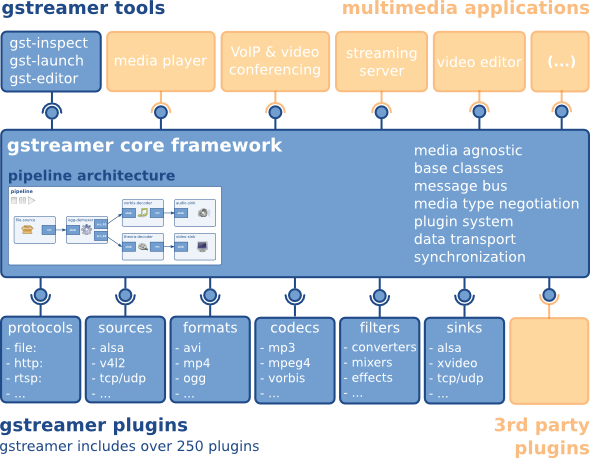
\includegraphics[scale=0.5]{figs/gstreamer-overview}
  \end{figure}
\end{frame}

\begin{frame}[c]{Dataflow}
  \begin{itemize}
    \item Dados são processados enquanto ``fluem" através de uma rede
    \item Estrutura de grafo dirigido
      \begin{itemize}
        \item Nós representam elementos de processamento (atores)
        \item Arestas representam conexões unidirecionais por onde fluem
          os dados
      \end{itemize}
    \item Atores recebem dados em portas de entrada e emitem dados através
      de portas de saída
    \item Um \en{pipeline} é um \en{dataflow} em que os dados fluem
      na mesma ordem em que foram produzidos
  \end{itemize}

  \begin{figure}[H]
    \centering
    \begin{tikzpicture}
      \node (filesrc) [element] {filesrc};
      \coordinate [above=.5\hdim of filesrc] (A);
      \coordinate [below=.5\hdim of filesrc] (B);
      %%
      \node (oggdemux) [element, right of=filesrc] {oggdemux};
      \coordinate [right of=oggdemux] (C);
      %%
      \node (vorbisdec) [element] at (C|-A) {vorbisdec};
      \node (alsasink) [element, right of=vorbisdec] {alsasink};
      \node (theoradec) [element] at (C|-B) {theoradec};
      \node (xvimagesink) [element, right of=theoradec] {xvimagesink};
      %%
      \draw [->, arrow] (filesrc) -- (oggdemux);
      \coordinate (X) at ($(oggdemux.east)+(0,.25\hdim)$);
      \coordinate (Y) at ($(oggdemux.east)+(0,-.25\hdim)$);
      \draw [->, arrow] (X) -- node [arrowlabel, above] {A} ++(\odim/3,0)
      -- ($(vorbisdec.west)-(\odim/3,0)$)
      -- (vorbisdec.west);
      \draw [->, arrow] (Y) -- node [arrowlabel, below] {V} ++(\odim/3,0)
      -- ($(theoradec.west)-(\odim/3,0)$)
      -- (theoradec.west);
      \draw [->, arrow] (vorbisdec) -- (alsasink);
      \draw [->, arrow] (theoradec) -- (xvimagesink);
    \end{tikzpicture}
  \end{figure}
\end{frame}

\begin{frame}[c]{Pipelines no GStreamer}
  \begin{itemize}
    \item Em um \en{pipeline} GStreamer os dados que fluem são tipicamente
      amostras de áudio e vídeo e dados de controle
    \item Nós do grafo (atores) são chamados elementos
    \item Portas por onde entram e saem dados dos elementos são chamados de
      \en{pads}
      \begin{itemize}
        \item \en{Sink pad} -- portas de entrada
        \item \en{Source pad} -- portas de saída
      \end{itemize}
    \item Tipos de elementos
      \begin{itemize}
        \item \en{Source} (produtores) -- possuem apenas \en{source pads}
        \item Processadores -- possuem \en{source} e \en{sink pads}
        \item \en{Sink} (consumidores) -- possuem apenas \en{sink pads}
      \end{itemize}
  \end{itemize}
\end{frame}

\begin{frame}[c]{Pipelines no GStreamer}
  Um \en{pipeline} GStreamer simplificado que reproduz um arquivo de
  vídeo Ogg.

  \begin{itemize}
    \item<2> \en{Source}
      \begin{itemize}
        \item filesrc
      \end{itemize}

    \item<3> Processadores
      \begin{itemize}
        \item oggdemux
        \item vorbisdec
        \item theoradec
      \end{itemize}

    \item<4> \en{Sinks}
      \begin{itemize}
        \item alsasink
        \item xvimagesink
      \end{itemize}
  \end{itemize}
  \newcommand*\overlaytwo{}
  \newcommand*\overlaythree{}
  \newcommand*\overlayfour{}
  \only<2>{\renewcommand*\overlaytwo{red}}
  \only<3>{\renewcommand*\overlaythree{red}}
  \only<4>{\renewcommand*\overlayfour{red}}

  \begin{figure}[h]
    \centering
    \begin{tikzpicture}
      \node (filesrc) [element, \overlaytwo] {filesrc};
      \coordinate [above=.5\hdim of filesrc] (A);
      \coordinate [below=.5\hdim of filesrc] (B);
      %%
      \node (oggdemux) [element, right of=filesrc, \overlaythree] {oggdemux};
      \coordinate [right of=oggdemux] (C);
      %%
      \node (vorbisdec) [element, \overlaythree] at (C|-A) {vorbisdec};
      \node (alsasink) [element, right of=vorbisdec, \overlayfour] {alsasink};
      \node (theoradec) [element, \overlaythree] at (C|-B) {theoradec};
      \node (xvimagesink) [element, right of=theoradec, \overlayfour] {xvimagesink};
      %%
      \draw [->, arrow] (filesrc) -- (oggdemux);
      \coordinate (X) at ($(oggdemux.east)+(0,.25\hdim)$);
      \coordinate (Y) at ($(oggdemux.east)+(0,-.25\hdim)$);
      \draw [->, arrow] (X) -- node [arrowlabel, above] {A} ++(\odim/3,0)
      -- ($(vorbisdec.west)-(\odim/3,0)$)
      -- (vorbisdec.west);
      \draw [->, arrow] (Y) -- node [arrowlabel, below] {V} ++(\odim/3,0)
      -- ($(theoradec.west)-(\odim/3,0)$)
      -- (theoradec.west);
      \draw [->, arrow] (vorbisdec) -- (alsasink);
      \draw [->, arrow] (theoradec) -- (xvimagesink);
    \end{tikzpicture}
  \end{figure}
\end{frame}

\begin{frame}[c]{Pipelines no GStreamer}
  \begin{block}{filesrc}
    Lê um arquivo do disco (vamos assumir um arquivo Ogg) e escreve o
    fluxo de bytes resultante na sua \en{source pad}
  \end{block}

  \begin{figure}
    \centering
    \begin{tikzpicture}
      \node (filesrc) [element, red] {filesrc};
      \coordinate [above=.5\hdim of filesrc] (A);
      \coordinate [below=.5\hdim of filesrc] (B);
      %%
      \node (oggdemux) [element, right of=filesrc] {oggdemux};
      \coordinate [right of=oggdemux] (C);
      %%
      \node (vorbisdec) [element] at (C|-A) {vorbisdec};
      \node (alsasink) [element, right of=vorbisdec] {alsasink};
      \node (theoradec) [element] at (C|-B) {theoradec};
      \node (xvimagesink) [element, right of=theoradec] {xvimagesink};
      %%
      \draw [->, arrow] (filesrc) -- (oggdemux);
      \coordinate (X) at ($(oggdemux.east)+(0,.25\hdim)$);
      \coordinate (Y) at ($(oggdemux.east)+(0,-.25\hdim)$);
      \draw [->, arrow] (X) -- node [arrowlabel, above] {A} ++(\odim/3,0)
      -- ($(vorbisdec.west)-(\odim/3,0)$)
      -- (vorbisdec.west);
      \draw [->, arrow] (Y) -- node [arrowlabel, below] {V} ++(\odim/3,0)
      -- ($(theoradec.west)-(\odim/3,0)$)
      -- (theoradec.west);
      \draw [->, arrow] (vorbisdec) -- (alsasink);
      \draw [->, arrow] (theoradec) -- (xvimagesink);
    \end{tikzpicture}
  \end{figure}
\end{frame}

\begin{frame}[c]{Pipelines no GStreamer}
  \begin{block}{oggdemux}
    Lê da sua \en{sink pad} um fluxo de bytes codificado no formato Ogg,
    demultiplexa-o e escreve os fluxos Vorbis (áudio) e Theora (vídeo)
    resultantes nas \en{source pads} correspondentes
  \end{block}

  \begin{figure}
    \centering
    \begin{tikzpicture}
      \node (filesrc) [element] {filesrc};
      \coordinate [above=.5\hdim of filesrc] (A);
      \coordinate [below=.5\hdim of filesrc] (B);
      %%
      \node (oggdemux) [element, right of=filesrc, red] {oggdemux};
      \coordinate [right of=oggdemux] (C);
      %%
      \node (vorbisdec) [element] at (C|-A) {vorbisdec};
      \node (alsasink) [element, right of=vorbisdec] {alsasink};
      \node (theoradec) [element] at (C|-B) {theoradec};
      \node (xvimagesink) [element, right of=theoradec] {xvimagesink};
      %%
      \draw [->, arrow] (filesrc) -- (oggdemux);
      \coordinate (X) at ($(oggdemux.east)+(0,.25\hdim)$);
      \coordinate (Y) at ($(oggdemux.east)+(0,-.25\hdim)$);
      \draw [->, arrow] (X) -- node [arrowlabel, above] {A} ++(\odim/3,0)
      -- ($(vorbisdec.west)-(\odim/3,0)$)
      -- (vorbisdec.west);
      \draw [->, arrow] (Y) -- node [arrowlabel, below] {V} ++(\odim/3,0)
      -- ($(theoradec.west)-(\odim/3,0)$)
      -- (theoradec.west);
      \draw [->, arrow] (vorbisdec) -- (alsasink);
      \draw [->, arrow] (theoradec) -- (xvimagesink);
    \end{tikzpicture}
  \end{figure}
\end{frame}

\begin{frame}[c]{Pipelines no GStreamer}
  \begin{block}{vorbisdec}
    Lê da sua \en{sink pad} um fluxo de bytes
    codificado no formato Vorbis, decodifica-o e escreve o fluxo de áudio~PCM
    resultante (áudio \en{raw} descomprimido) na sua \en{source pad}
  \end{block}

  \begin{figure}
    \centering
    \begin{tikzpicture}
      \node (filesrc) [element] {filesrc};
      \coordinate [above=.5\hdim of filesrc] (A);
      \coordinate [below=.5\hdim of filesrc] (B);
      %%
      \node (oggdemux) [element, right of=filesrc] {oggdemux};
      \coordinate [right of=oggdemux] (C);
      %%
      \node (vorbisdec) [element, red] at (C|-A) {vorbisdec};
      \node (alsasink) [element, right of=vorbisdec] {alsasink};
      \node (theoradec) [element] at (C|-B) {theoradec};
      \node (xvimagesink) [element, right of=theoradec] {xvimagesink};
      %%
      \draw [->, arrow] (filesrc) -- (oggdemux);
      \coordinate (X) at ($(oggdemux.east)+(0,.25\hdim)$);
      \coordinate (Y) at ($(oggdemux.east)+(0,-.25\hdim)$);
      \draw [->, arrow] (X) -- node [arrowlabel, above] {A} ++(\odim/3,0)
      -- ($(vorbisdec.west)-(\odim/3,0)$)
      -- (vorbisdec.west);
      \draw [->, arrow] (Y) -- node [arrowlabel, below] {V} ++(\odim/3,0)
      -- ($(theoradec.west)-(\odim/3,0)$)
      -- (theoradec.west);
      \draw [->, arrow] (vorbisdec) -- (alsasink);
      \draw [->, arrow] (theoradec) -- (xvimagesink);
    \end{tikzpicture}
  \end{figure}
\end{frame}

\begin{frame}[c]{Pipelines no GStreamer}
  \begin{block}{theoradec}
    Lê da sua \en{sink pad} um fluxo de bytes codificado no formato
    Theora, decodifica-o e escreve o fluxo de vídeo \en{raw} descomprimido
    resultante na sua \en{source pad}
  \end{block}

  \begin{figure}
    \centering
    \begin{tikzpicture}
      \node (filesrc) [element] {filesrc};
      \coordinate [above=.5\hdim of filesrc] (A);
      \coordinate [below=.5\hdim of filesrc] (B);
      %%
      \node (oggdemux) [element, right of=filesrc] {oggdemux};
      \coordinate [right of=oggdemux] (C);
      %%
      \node (vorbisdec) [element] at (C|-A) {vorbisdec};
      \node (alsasink) [element, right of=vorbisdec] {alsasink};
      \node (theoradec) [element, red] at (C|-B) {theoradec};
      \node (xvimagesink) [element, right of=theoradec] {xvimagesink};
      %%
      \draw [->, arrow] (filesrc) -- (oggdemux);
      \coordinate (X) at ($(oggdemux.east)+(0,.25\hdim)$);
      \coordinate (Y) at ($(oggdemux.east)+(0,-.25\hdim)$);
      \draw [->, arrow] (X) -- node [arrowlabel, above] {A} ++(\odim/3,0)
      -- ($(vorbisdec.west)-(\odim/3,0)$)
      -- (vorbisdec.west);
      \draw [->, arrow] (Y) -- node [arrowlabel, below] {V} ++(\odim/3,0)
      -- ($(theoradec.west)-(\odim/3,0)$)
      -- (theoradec.west);
      \draw [->, arrow] (vorbisdec) -- (alsasink);
      \draw [->, arrow] (theoradec) -- (xvimagesink);
    \end{tikzpicture}
  \end{figure}
\end{frame}

\begin{frame}[c]{Pipelines no GStreamer}
  \begin{block}{alsasink}
    Lê um fluxo de áudio descomprimido da sua \en{sink pad} e utiliza
    a biblioteca ALSA para reproduzir as amostras do fluxo
    nos alto-falantes
  \end{block}

  \begin{figure}
    \centering
    \begin{tikzpicture}
      \node (filesrc) [element] {filesrc};
      \coordinate [above=.5\hdim of filesrc] (A);
      \coordinate [below=.5\hdim of filesrc] (B);
      %%
      \node (oggdemux) [element, right of=filesrc] {oggdemux};
      \coordinate [right of=oggdemux] (C);
      %%
      \node (vorbisdec) [element] at (C|-A) {vorbisdec};
      \node (alsasink) [element, right of=vorbisdec, red] {alsasink};
      \node (theoradec) [element] at (C|-B) {theoradec};
      \node (xvimagesink) [element, right of=theoradec] {xvimagesink};
      %%
      \draw [->, arrow] (filesrc) -- (oggdemux);
      \coordinate (X) at ($(oggdemux.east)+(0,.25\hdim)$);
      \coordinate (Y) at ($(oggdemux.east)+(0,-.25\hdim)$);
      \draw [->, arrow] (X) -- node [arrowlabel, above] {A} ++(\odim/3,0)
      -- ($(vorbisdec.west)-(\odim/3,0)$)
      -- (vorbisdec.west);
      \draw [->, arrow] (Y) -- node [arrowlabel, below] {V} ++(\odim/3,0)
      -- ($(theoradec.west)-(\odim/3,0)$)
      -- (theoradec.west);
      \draw [->, arrow] (vorbisdec) -- (alsasink);
      \draw [->, arrow] (theoradec) -- (xvimagesink);
    \end{tikzpicture}
  \end{figure}
\end{frame}

\begin{frame}[c]{Pipelines no GStreamer}
  \begin{block}{xvimagesink}
    Lê um fluxo de vídeo descomprimido da sua \en{sink pad} e utiliza
    a biblioteca X11 para reproduzir os quadros do fluxo na tela
  \end{block}

  \begin{figure}
    \centering
    \begin{tikzpicture}
      \node (filesrc) [element] {filesrc};
      \coordinate [above=.5\hdim of filesrc] (A);
      \coordinate [below=.5\hdim of filesrc] (B);
      %%
      \node (oggdemux) [element, right of=filesrc] {oggdemux};
      \coordinate [right of=oggdemux] (C);
      %%
      \node (vorbisdec) [element] at (C|-A) {vorbisdec};
      \node (alsasink) [element, right of=vorbisdec] {alsasink};
      \node (theoradec) [element] at (C|-B) {theoradec};
      \node (xvimagesink) [element, right of=theoradec, red] {xvimagesink};
      %%
      \draw [->, arrow] (filesrc) -- (oggdemux);
      \coordinate (X) at ($(oggdemux.east)+(0,.25\hdim)$);
      \coordinate (Y) at ($(oggdemux.east)+(0,-.25\hdim)$);
      \draw [->, arrow] (X) -- node [arrowlabel, above] {A} ++(\odim/3,0)
      -- ($(vorbisdec.west)-(\odim/3,0)$)
      -- (vorbisdec.west);
      \draw [->, arrow] (Y) -- node [arrowlabel, below] {V} ++(\odim/3,0)
      -- ($(theoradec.west)-(\odim/3,0)$)
      -- (theoradec.west);
      \draw [->, arrow] (vorbisdec) -- (alsasink);
      \draw [->, arrow] (theoradec) -- (xvimagesink);
    \end{tikzpicture}
  \end{figure}
\end{frame}

\begin{frame}[c]{Sincronização}
  \begin{itemize}
    \item \en{Pipelines} possuem um relógio para controlar a sincronização
      dos fluxos
    \item Cada amostra de áudio e vídeo possuem um tempo de apresentação
      (PTS -- \en{presentation timestamp}) e uma duração
    \item Elementos \en{sink} controlam a taxa de reprodução de cada
      fluxo
      \begin{itemize}
        \item Amostras recebidas antes do seu tempo de apresentação são
          armazenadas em uma fila interna para serem exibidas no
          tempo adequado
        \item Amostras recebidas após o seu tempo de apresentação são
          descartadas
      \end{itemize}
    \item Todos os outros elementos do \en{pipeline} operam livremente
      \begin{itemize}
        \item Consumem e produzem dados em taxas arbitrárias
      \end{itemize}
  \end{itemize}
\end{frame}

\begin{frame}[c]{Pads}
  \begin{itemize}
    \item \en{Pads} são pontos de conexão entre elementos
      \begin{itemize}
        \item source $\rightarrow$ sink \textcolor{green}{\checkmark}
        \item sink $\rightarrow$ source $\color{red}{\times}$
      \end{itemize}
    \item Dois tipos de dados trafegam entre \en{pads}
      \begin{itemize}
        \item Dados (\en{buffers})
          \begin{itemize}
            \item Amostras de áudio/vídeo
            \item Fluem exclusivamente na direção das conexões
          \end{itemize}
        \item Eventos (\en{events})
          \begin{itemize}
            \item Informações de controle
            \item Podem fluir em ambos os sentidos das conexões
            \item Ex: QoS, seek, flush, \ldots
          \end{itemize}
      \end{itemize}
    \item Dados e eventos podem percorrer as conexões em paralelo
  \end{itemize}

  \begin{figure}[H]
    \centering
    \begin{tikzpicture}
      \node [cylinder, thick, draw=black!60, cylinder uses custom fill,
      cylinder end fill=black!30, cylinder body fill=black!20,
      minimum height=\wdim, minimum width=\hdim] (c) {};
      \coordinate (x) at ($(c.before top|-c.east)+(0,.15\hdim)$);
      \coordinate (y) at ($(c.before top|-c.east)-(0,.15\hdim)$);
      \coordinate (x0) at ($(c.west|-x)+(.25pt,0)$);
      \coordinate (y0) at ($(c.west|-y)+(.25pt,0)$);
      \draw [->,arrow] (x)
      -- node [arrowlabel, above, pos=.4] {B} ++(\odim,0);
      \draw [arrow] (x0) -- ++(-\odim,0);
      \draw [->,arrow] (y)
      -- node [arrowlabel, below, pos=.4] {E} ++(\odim,0);
      \draw [->,arrow] (y0) -- ++(-\odim,0);
    \end{tikzpicture}
  \end{figure}
  \vskip-\baselineskip
  Estrutura conceitual de uma conexão entre \en{pads} no
  GStreamer.
\end{frame}

\begin{frame}[c]{Bins -- Agrupando Elementos em Contêineres}
  \begin{figure}
    \centering
    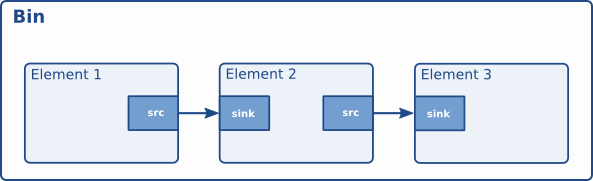
\includegraphics[scale=0.5]{figs/bin}
  \end{figure}

  \begin{itemize}
    \item Bins são contêineres que agrupam elementos
      \begin{itemize}
        \item \en{Pipelines} também são \en{bins}
      \end{itemize}
    \item Dois elementos só podem ser ligados se e somente se eles estiverem
      dentro do mesmo contêiner
  \end{itemize}
\end{frame}

\begin{frame}[c]{Bus -- Barramento de Comunicação}
  \begin{figure}
    \centering
    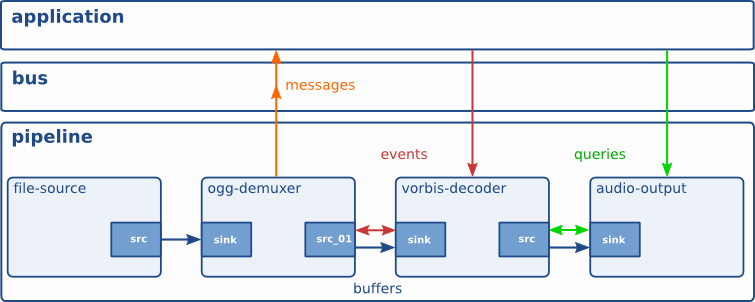
\includegraphics[scale=0.5]{figs/bus}
  \end{figure}

  \begin{itemize}
    \item Elementos postam mensagens no barramento de comunicação (\en{bus})
      para se comunicarem com a aplicação
  \end{itemize}
\end{frame}

\section{Hands on}
\subsection{Olá Mundo}

\begin{frame}[fragile]{Primeira Aplicação: Olá mundo}
  Tocando um vídeo no GStreamer usando o elemento ``playbin''.
  \begin{itemize}
    \item Arquivo: src/hello.c
  \end{itemize}
  ~

  Compilando o código fonte hello.c:
  \begin{lstlisting}[style=command]
  $ cc hello.c -o hello `pkg-config --cflags --libs
        glib-2.0 gstreamer-1.0`
  \end{lstlisting}
\end{frame}

\subsection{Player MP3}

\begin{frame}[c]{Tocando um Arquivo MP3}
  Player MP3.
  \begin{figure}[t]
    \centering
    \begin{tikzpicture}
      \node (filesrc) [element] {filesrc};
      \node (mad) [element, right of=filesrc] {mad};
      \node (alsasink) [element, right of=mad] {alsasink};
      \coordinate (A) at ($(filesrc.north west)+(-.5\odim,.5\odim)$);
      \coordinate (B) at ($(alsasink.south east)+(.5\odim,-.5\odim)$);
      \path [bin] (A) rectangle node [binlabel] {pipeline} (B);
      \draw [->, arrow] (filesrc) -- (mad);
      \draw [->, arrow] (mad) -- (alsasink);
    \end{tikzpicture}
  \end{figure}
  \en{Pipeline} que reproduz um arquivo de áudio~MP3.
  ~
  \begin{itemize}
    \item Arquivo: src/mp3.c
  \end{itemize}
\end{frame}

\begin{frame}[c]{Máquinas de Estado de um GstElement}
  \begin{itemize}
    \item Todo elemento possui um estado, que pode ser:
      \begin{itemize}
        \item GST\_STATE\_NULL (nulo)
        \item GST\_STATE\_READY (pronto)
        \item GST\_STATE\_PAUSED (pausado)
        \item GST\_STATE\_PLAYING (tocando)
      \end{itemize}
    \item Mudanças de estado são propagadas para elementos filhos (\en{bins})
      \begin{itemize}
        \item Direção de propagação é sempre dos \en{sinks} para
          os \en{sources}
        \item Isso evita que dados sejam gerados antes que elementos
          posteriores no \en{pipeline} estejam prontos para recebê-los
      \end{itemize}
  \end{itemize}

  \begin{figure}[h]
    \centering
    \begin{tikzpicture}[node distance=1.5\hdim+\odim]
      \node [state] (NULL) {null};
      \node [state, right of=NULL] (READY) {ready};
      \node [state, right of=READY] (PAUSED) {paused};
      \node [state, right of=PAUSED] (PLAYING) {playing};
      \draw [->] (NULL) to [bend left=20] (READY);
      \draw [->] (READY) to [bend left=20] (PAUSED);
      \draw [->] (PAUSED) to [bend left=20] (PLAYING);
      \draw [->] (PLAYING) to [bend left=20] (PAUSED);
      \draw [->] (PAUSED) to [bend left=20] (READY);
      \draw [->] (READY) to [bend left=20] (NULL);
    \end{tikzpicture}
  \end{figure}
\end{frame}

\subsection{Player Ogg}

\begin{frame}[c]{Um pouco mais sobre \en{pads}}
  Cada \en{pad} possui três atributos importantes de serem considerados
  para ligar dois elementos
  \begin{itemize}
    \item<2-> Direção
      \begin{itemize}
        \item \en{Sink}
        \item \en{Source}
      \end{itemize}
    \item<3-> Capacidade
      \begin{itemize}
        \item \en{Caps} -- determina os tipos de \en{buffers} que podem
          atravessá-la
      \end{itemize}
    \item<4-> Disponibilidade
      \begin{itemize}
        \item \en{Always} (sempre)
        \item \en{Sometimes} (às vezes)
        \item \en{Request} (sob requisição)
      \end{itemize}
  \end{itemize}
\end{frame}

\begin{frame}[c]{Disponibilidade de \en{Pads}}
  \begin{itemize}
    \item<1-> \en{Always}
      \begin{itemize}
        \item Criadas assim que o elemento é criado
        \item \C{gst_element_get_static_pad ()}
      \end{itemize}
    \item<2-> \en{Sometimes}
      \begin{itemize}
        \item Criada pelo próprio elemento sob condições específicas que
          normalmente envolvem o conteúdo processado
      \end{itemize}
    \item<3-> \en{Request}
      \begin{itemize}
        \item Criada apenas quando requisitadas pela aplicação
        \item \C{gst_element_get_request_pad()}
      \end{itemize}
  \end{itemize}
\end{frame}

\begin{frame}[c]{Tocando um Arquivo Ogg}
  Pipeline de um player Ogg
  \begin{adjustbox}{max totalsize={.9\textwidth}{\textheight},center}
    \begin{tikzpicture}
      \node (filesrc) [element] {filesrc};
      \coordinate [above=.5\hdim of filesrc] (A);
      \coordinate [below=.5\hdim of filesrc] (B);
      %%
      \node (oggdemux) [element, right of=filesrc] {oggdemux};
      \coordinate [right of=oggdemux] (C);
      %%
      \node (vorbisdec) [element] at (C|-A) {vorbisdec};
      \node (audioconvert) [element, right of=vorbisdec] {audioconvert};
      \node (alsasink) [element, right of=audioconvert] {alsasink};
      \node (queue) [element] at (C|-B) {queue};
      \node (theoradec) [element, right of=queue] {theoradec};
      \node (xvimagesink) [element, right of=theoradec] {xvimagesink};
      %%
      \draw [->, arrow] (filesrc) -- (oggdemux);
      \coordinate (X) at ($(oggdemux.east)+(0,.25\hdim)$);
      \coordinate (Y) at ($(oggdemux.east)+(0,-.25\hdim)$);
      \draw [->, arrow] (X) -- node [arrowlabel, above] {A} ++(\odim/3,0)
      -- ($(vorbisdec.west)-(\odim/3,0)$)
      -- (vorbisdec.west);
      \draw [->, arrow] (Y) -- node [arrowlabel, below] {V} ++(\odim/3,0)
      -- ($(queue.west)-(\odim/3,0)$)
      -- (queue.west);
      \draw [->, arrow] (vorbisdec) -- (audioconvert);
      \draw [->, arrow] (audioconvert) -- (alsasink);
      \draw [->, arrow] (queue) -- (theoradec);
      \draw [->, arrow] (theoradec) -- (xvimagesink);
    \end{tikzpicture}
  \end{adjustbox}
  \begin{itemize}
    \item Um contêiner Ogg pode conter múltiplos fluxos multiplexados
    \item O demultiplexador \en{oggdemux} cria \en{source pads} para
      cada fluxo multiplexado no arquivo
      \begin{itemize}
        \item \en{Source pads} possuem disponibilidade \en{sometimes}
      \end{itemize}
    \item Só podemos conectar o elemento \en{oggdemux} ao resto do
      \en{pipeline} quando as \en{source pads} forem criadas
    \item Notificação assíncrona (sinais)
      \begin{itemize}
        \item O elemento \en{oggdemux} emite o sinal \en{pad-added} sempre
          que uma nova \en{source pad} é criada
      \end{itemize}
  \end{itemize}
\end{frame}

\begin{frame}[c]{Tocando um Arquivo Ogg}
  Player Ogg:
  \begin{itemize}
    \item Arquivo: src/ogg2.c
  \end{itemize}
\end{frame}

\subsection{Comandos gst-launch e gst-inspect}
\begin{frame}[fragile]{gst-launch}
  \begin{itemize}
    \item Permite construir pipelines estáticos (que não mudam após montados) tipo diretamente na linha de comando
    \item Particularmente útil para depurar ou testar a
      viabilidade de \en{pipelines} antes de implementá-los em C
    \item Em algumas instalações o nome do comando é \C{gst-launch-1.0}
  \end{itemize}

  \begin{lstlisting}[style=command,breaklines=true]
gst-launch playbin uri="file://$PWD/bunny.ogg"
gst-launch filesrc location=bunny.mp3 ! mad ! alsasink
gst-launch filesrc location=bunny.ogg ! oggdemux name=demux\
   demux. ! vorbisdec ! audioconvert ! alsasink\
   demux. ! queue     ! theoradec    ! xvimagesink
 \end{lstlisting}
\end{frame}

\begin{frame}[fragile]{Um \en{Pipeline} Genérico}
  \begin{lstlisting}[style=command,breaklines=true]
gst-launch uridecodebin uri="<URI>" name=decbin\
  decbin.@@ ! audioconvert ! autoaudiosink\
  decbin.@@ ! autovideosink
 \end{lstlisting}

 \begin{figure}[H]
   \centering
   \begin{tikzpicture}
     \node (uridecodebin) [element] {uridecodebin};
     \coordinate [above=.5\hdim of uridecodebin] (A);
     \coordinate [below=.5\hdim of uridecodebin] (B);
     %%
     \coordinate [right of=uridecodebin] (C);
     \node (audioconvert) [element] at (C|-A) {audioconvert};
     \node (autoaudiosink) [element, right of=audioconvert] {autoaudiosink};
     %%
     \coordinate [right of=audioconvert] (D);
     \node (autovideosink) [element] at (D|-B) {autovideosink};
     %%
     \coordinate (X) at ($(uridecodebin.east)+(0,.25\hdim)$);
     \coordinate (Y) at ($(uridecodebin.east)+(0,-.25\hdim)$);
     \draw [->, arrow] (X) -- node [arrowlabel, above] {A} ++(\odim/3,0)
     -- ($(audioconvert.west)-(\odim/3,0)$)
     -- (audioconvert.west);
     \draw [->, arrow] (Y) -- node [arrowlabel, below] {V} ++(\odim/3,0)
     -- ($(audioconvert.west|-B)-(\odim/3,0)$)
     -- (autovideosink.west);
     \draw [->, arrow] (audioconvert) -- (autoaudiosink);
   \end{tikzpicture}
 \end{figure}
\end{frame}

\begin{frame}[fragile]{gst-inspect}
  \begin{itemize}
    \item Permite inspecionar os \en{plugins} e elementos disponíveis
      no sistema
    \item Em algumas instalações o nome do comando é \en{gst-inspect-1.0}
  \end{itemize}

  Exemplo: \$ gst-inspect equalizer

  \lstinputlisting[
  language={},
  style=display,
  ]{../src/equalizer.out}
\end{frame}

\subsection{Filtros}
\begin{frame}[fragile]{Filtros}
  \begin{itemize}
    \item Aplicam transformações sobre um fluxo de amostras descomprimidas
    \item Altera o fluxo original, produzindo efeitos sonoros ou visuais
  \end{itemize}
  ~
  Alguns filtros de áudio e vídeo disponíveis no GStreamer:
  \begin{table}[h]
    \sffamily
    \scriptsize
    \centering
    \begin{tabular}{llll}
      \toprule
      &\textbf{Plugin}
      &\textbf{Elemento}
      &\textbf{Descrição (controle)}\\
      \midrule
      \textbf{Áudio}
      &audiofx    & audiodynamic & Compressão ou expansão\\
      &audiofx    & audioecho    & Eco\\
      &equalizer  & equalizer-nbands& Equalização~($n$~bandas)\\
      &freeverb   & freeverb     & Reverberação\\
      &soundtouch & pitch        & Tonalidade e tempo\\
      &speed      & speed        & Velocidade\\
      &volume     & volume       & Volume\\
      \multicolumn{4}{l}{\dotfill}\\
      \textbf{Vídeo}
      &coloreffects& coloreffects& Efeito de colorização\\
      &effectv     & revtv       & Efeito de relevo\\
      &effectv     & shagadelictv& Efeito de espiral caleidoscópica\\
      &videocrop   & videocrop   & Recorte\\
      &videofilter & videobalance& Brilho, cor e saturação\\
      &videoscale  & videoscale  & Redimensionamento\\
      \bottomrule
    \end{tabular}
  \end{table}
\end{frame}

\begin{frame}[fragile]{Aplicando filtros}
  Exemplo simples usando gst-launch:
  \begin{lstlisting}[style=command]
$ gst-launch filesrc location=bunny.mp3\
      ! mad ! volume volume=.5 ! alsasink
  \end{lstlisting}
\end{frame}

\begin{frame}[c]{Aplicando filtros}
  Exemplo mais complexo:

  \begin{adjustbox}{max totalsize={.9\textwidth}{\textheight},center}
    \begin{tikzpicture}
      \node (uridecodebin) [element] {uridecodebin};
      \coordinate [above=.5\hdim of uridecodebin] (A);
      \coordinate [below=.5\hdim of uridecodebin] (B);
      %%
      \coordinate [right of=uridecodebin] (C);
      \node (videoconvert1) [element] at (C|-B) {videoconvert};
      \node (videofilter) [element, right of=videoconvert1]
      {$\<\text{\emph{video filter}}>$};
      \node (videoconvert2) [element, right of=videofilter] {videoconvert};
      \node (autovideosink) [element, right of=videoconvert2] {autovideosink};
      %%
      \coordinate [above of=videofilter] (D);
      \node (audiofilter) [element] at (D|-A)
      {$\<\text{\emph{audio filter}}>$};
      \node (audioconvert) [element, right of=audiofilter] {audioconvert};
      \node (autoaudiosink) [element, right of=audioconvert] {autoaudiosink};
      %%
      \coordinate (X) at ($(uridecodebin.east)+(0,.25\hdim)$);
      \coordinate (Y) at ($(uridecodebin.east)+(0,-.25\hdim)$);
      \draw [->, arrow] (X) -- node [arrowlabel, above] {A} ++(\odim/3,0)
      -- ($(videoconvert1.west|-A)-(\odim/3,0)$)
      -- (audiofilter.west);
      \draw [->, arrow] (Y) -- node [arrowlabel, below] {V} ++(\odim/3,0)
      -- ($(videoconvert1.west)-(\odim/3,0)$)
      -- (videoconvert1.west);
      \draw [->, arrow] (audiofilter) -- (audioconvert);
      \draw [->, arrow] (audioconvert) -- (autoaudiosink);
      \draw [->, arrow] (videoconvert1) -- (videofilter);
      \draw [->, arrow] (videofilter) -- (videoconvert2);
      \draw [->, arrow] (videoconvert2) -- (autovideosink);
    \end{tikzpicture}
  \end{adjustbox}

  \begin{itemize}
    \item Arquivo: src/filter.c
  \end{itemize}
\end{frame}

\begin{frame}[c]{Aplicando filtros}
  Efeitos de vídeo aplicados pelo programa anterior:
  \begin{figure}[h]
    \centering
    \subfigure[Quadro original.]{
      
\includegraphics[width=0.3\textwidth]{../media/bird}
    }
    \subfigure[Filtro ``coloreffects''.]{
      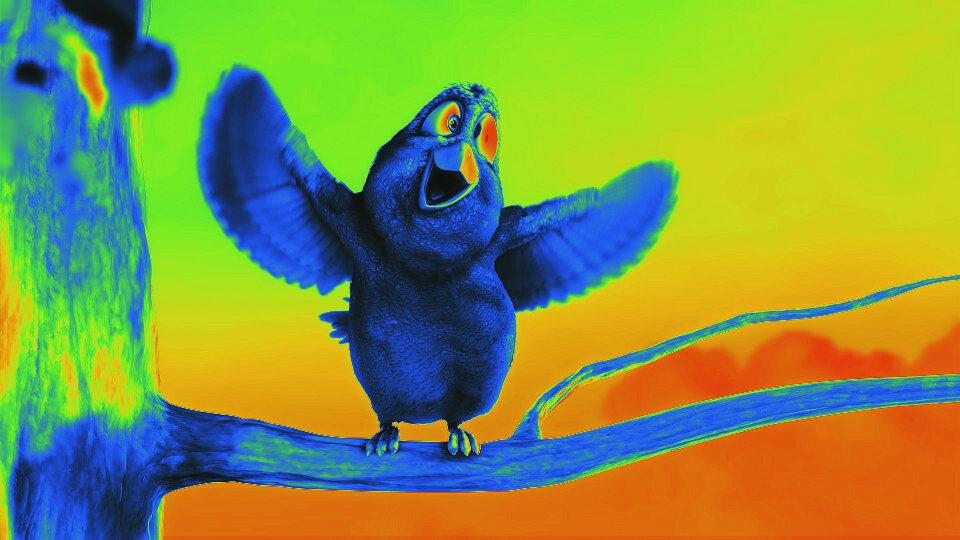
\includegraphics[width=0.3\textwidth]{../media/bird-coloreffects}
    }
    \subfigure[Filtro ``dicetv''.]{
      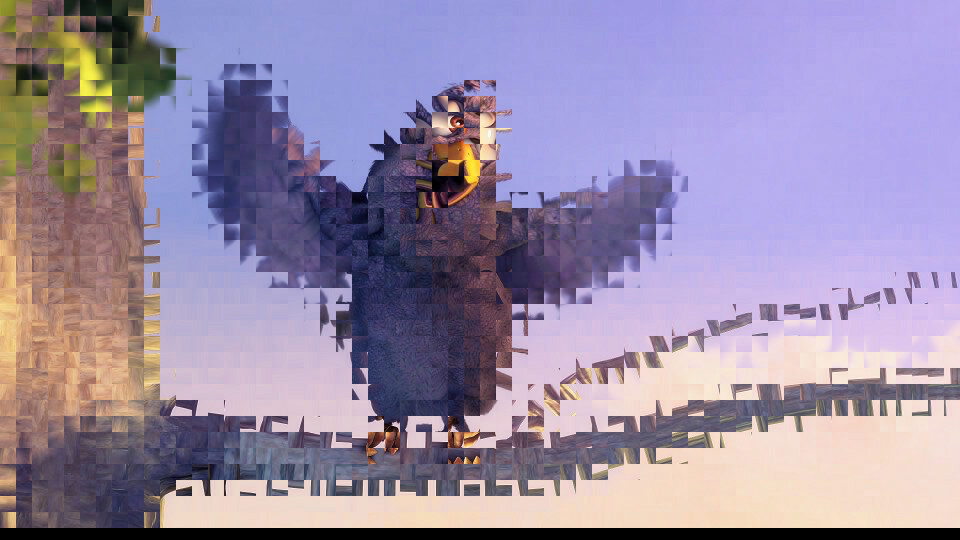
\includegraphics[width=0.3\textwidth]{../media/bird-dicetv}
    }
    \subfigure[Filtro ``shagadelictv''.]{
      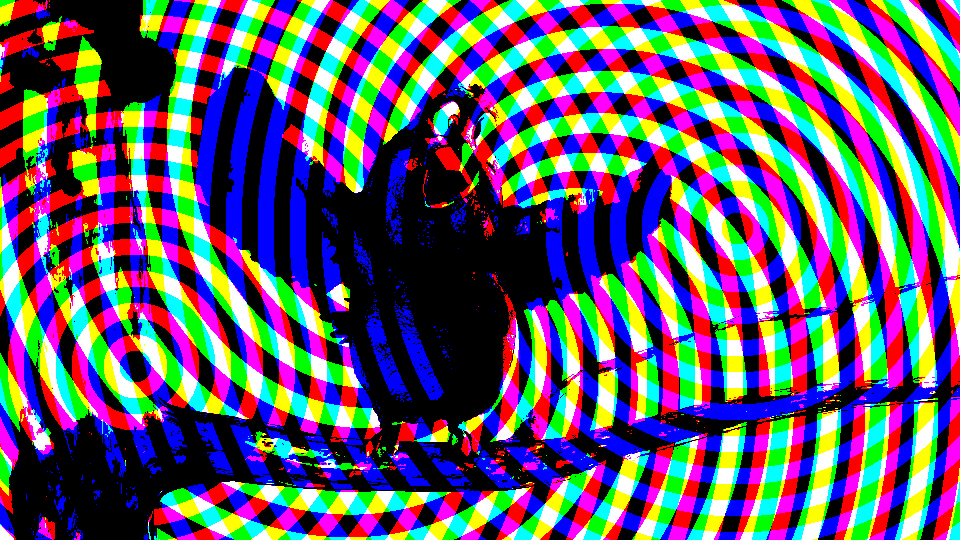
\includegraphics[width=0.3\textwidth]{../media/bird-shagadelictv}
    }
    \subfigure[Filtro ``edgetv''.]{
      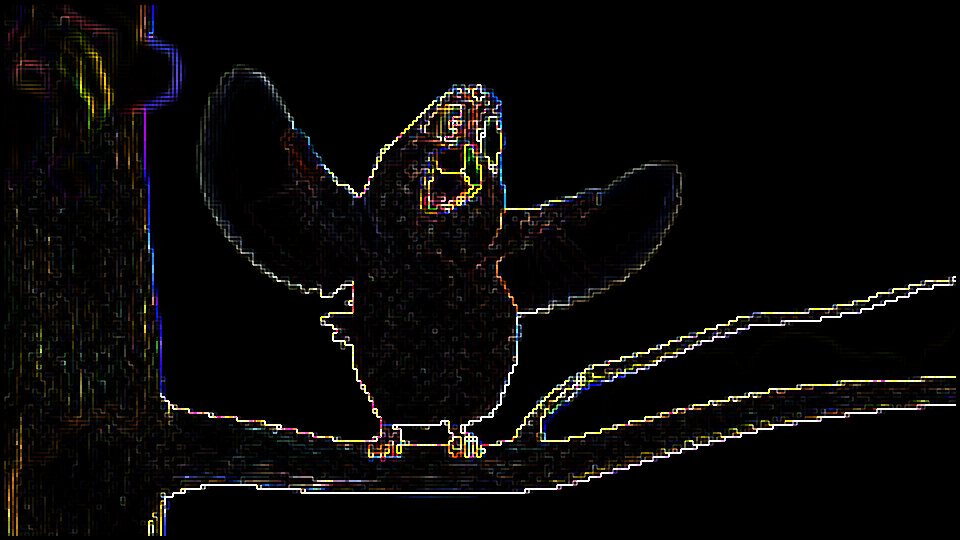
\includegraphics[width=0.3\textwidth]{../media/bird-edgetv}
    }
    \subfigure[Filtro ``revtv''.]{
      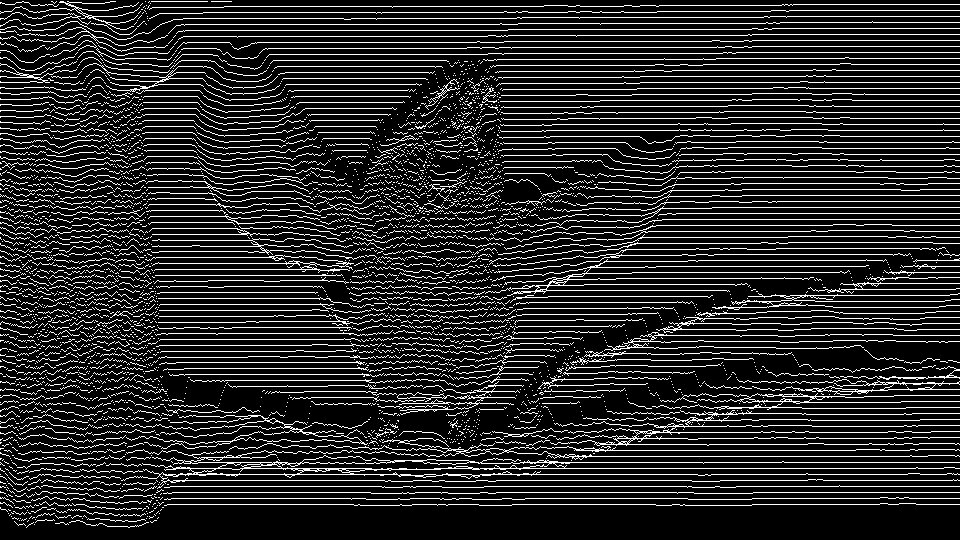
\includegraphics[width=0.3\textwidth]{../media/bird-revtv}
    }
  \end{figure}
\end{frame}

\subsection{Play, pause, stop, seek, fast-forward, rewind}
\begin{frame}[c]{Controles avançados}
  Vamos incrementar o programa ``Olá mundo'' para que ele responda aos
  seguintes comandos:

  \begin{center}
    \begin{tabular}{cl}
      \keystroke{SPC} & pausa ou resume a reprodução
      (\en{pause} e \en{play})\\[2\jot]
      \keystroke{$\to$} & avança~5s (\en{seek})\\[2\jot]
      \keystroke{$\leftarrow$} & retrocede~5s (\en{seek})\\[2\jot]
      \keystroke{F} & reproduz~2x mais rápido (\en{fast-foward})\\[2\jot]
      \keystroke{R} & reproduz ao contrário~2x mais rápido
      (\en{rewind})\\[2\jot]
      \keystroke{N} & reproduz na velocidade original\\[2\jot]
      \keystroke{Q} & para a reprodução e termina o programa (\en{stop})
    \end{tabular}
  \end{center}
\end{frame}

\begin{frame}[c]{Controles avançados}
  \begin{itemize}
    \item Elementos \en{sink} postam mensagens de eventos de navegação
      \C{GST_NAVIGATION_MESSAGE_EVENT} no \en{bus} para informar eventos
      de tecla e de mouse
    \item A postagem de eventos de \en{seek} (\C{GST_EVENT_SEEK}) requisitam
      mudanças na posição e na taxa de reprodução de um fluxo
    \item Arquivo: src/controls.c
  \end{itemize}
\end{frame}

\end{document}
